\chapter{Floating-Point Arithmetic}\index{floating-point arithmetic}
\newthought{Getting used to Errors Everywhere}


% Bring a better visualization of where the points fall in a 1 Bit mantissa, 
% then show how the gaps between representable numbers grow as the exponent increases, 
% then show how many values we can have with a limited exponent. 
% then show how we can use the same number and use it in a range limited fixed-point style. 


% Einfluss Mantisse und Exponent deutlich zeigen an Beispielen. 1 Bit jeweils, dann 2 und 1 Bit in Gruppen.
% Dann zeigen wie die Lücken zwischen den Zahlen wachsen, wenn der Exponent größer wird.
% Dann überleiten auf Fixed Point

% Maschinenfehler am Taschenrechner bestimmen lassen.
% Dann zeigen wie Maschinenfehler und Loss of Significance zusammenhängen .. . hier schwimmt es noch. 

% ==============================================================================================
% INTRODUCTION BLOCK - 15 minutes

\section{The Why}

\marginnote{\newthought{Modeling Error}\index{modeling error} occurs as all models are simplifications of reality, and the difference between the model and the real-world system introduces an error. 
We will not dive deeper into this type of error in this course. Yet, mind the fine difference between what we term $f(x)$ and what actually is a $\tilde{f(x)}$.}

\newthought{We saw that} numerical methods introduce errors through approximation. 

Where $f(x)$ be a continuous function on $[a, b]$. The discretized version $f(x_i)$ approximates $f(x)$ at discrete points $x_i$ with an error that
depends on the step size $h$ and the smoothness of $f$. 
Numerical values can further only be stored approximately in a computer's memory, in floating-point representation\index{floating-point representation}.
This leads to rounding errors\index{rounding error} when performing arithmetic operations, adding up to the truncation errors\index{truncation error} we already experienced when approximating infinite processes with finite ones, it is also called approximation error.

\newthought{This gives us good reason} to understand these errors and their interplay with our machines.
\begin{itemize}
    \item Numerical methods introduce rounding\index{rounding error} and truncation errors\index{truncation error}.
    \item Based on our machines these errors play out differently, and can amplify and accumulate.\index{numerical stability}
\end{itemize} 


\marginnote{

\newthought{On the Edge} models use lower-precision arithmetic, 
such as 8-bit integers or even binary weights and activations.\\
\newthought{Binary neural networks} (BNNs) use weights and activations constrained to $\{-1, +1\}$, drastically reducing memory and computation requirements, but making floating-point representation\index{floating-point representation} and rounding effects\index{rounding error} critical.
}

\newthought{In machine learning and artificial intelligence,} you already are aware thatnumerical methods are crucial for training models, but of course floating-point arithmetic

is as relevant in model inference. Especially in compute-sparse environments on the edge, or when deploying quantized models \cite{courbariauxbnn}, understanding floating-point arithmetic\index{floating-point arithmetic} and the underlying mechanics comes handy.





\newpage
\subsection{Hands On Experience}

Let's get a feeling for rounding error\index{rounding error} with a simple example.

\newthought{Consider dividing $10$ by $3$}. Write out the decimal expansion:
\begin{align*}
    &10 \div 3 = 3 \quad \text{remainder: } 1 \\
    &\text{Bring down a 0: } 10 \div 3 = 3 \quad \text{remainder: } 1 \\
    &\text{Bring down a 0: } 10 \div 3 = 3 \quad \text{remainder: } 1 \\
    &\text{Bring down a 0: } 10 \div 3 = 3 \quad \text{remainder: } 1 \\
    &\text{... and so on} \\
    &\Rightarrow \frac{10}{3} = 3.333\ldots
\end{align*}


\marginnote{
\newthought{Types} of numerical representations in computers include: \\
\textbf{Integer} (int):\\
$3$ \\
\textbf{Floating-point} (float):\\
$3.3333333$ \\
\textbf{Double precision} (double):\\
$3.3333333333333333$ \\
\textbf{Fixed-point} (e.g. 4-digits):\\
$3.3333$\index{fixed-point representation}
}

\newthought{The $3$s repeat forever}. But when you write it down or enter it into a calculator or computer, you have to stop at some point:
\begin{equation}
    \frac{10}{3} \approx 3.333 \quad \text{(rounded or truncated after 3 digits)}
\end{equation}
What you will end up with is the rounding error: The difference between the true value and the value you get when you cut off (truncate) the expansion.
No matter how many digits you write, as soon as you stop, you introduce an error:
\begin{equation}
    \text{Rounding error} = \left|\, 3.333333\ldots - 3.333\, \right| = 0.000333\ldots
\end{equation}

The more digits you keep, the smaller the error, but it never disappears completely unless you write infinitely many digits, which well, you know is impossible.
\marginnote{\newthought{Impossible?} Mathematical annotation helps us with period: $3.\overline{3}$.}

\newthought{This is rounding error:} Computers always store numbers with a finite number of digits, so rounding errors will inevitably show up and need to be managed.

Because as you will see, these small errors can accumulate and amplify and lead to significant inaccuracies in computations, especially in iterative algorithms common in numerical methods and machine learning.\index{numerical stability}

\newthought{The Learning Objectives} of this chapter aim at providing you with the abilities to:
\begin{itemize}
    \item Understand the different types of numerical errors: Modeling\index{modeling error}, truncation\index{truncation error}, and rounding errors\index{rounding error}.
    \item Comprehend floating-point representation\index{floating-point representation}, machine epsilon\index{machine epsilon}, and loss of significance\index{loss of significance}.
    \item Be able to handle numerical errors in practical computations.\index{numerical stability}
\end{itemize}






























% ==============================================================================================
% MAIN THEORY BLOCK - 15 minutes

\newpage
\section{Floating Point Representation and Precision}


\newthought{Floating-point numbers}\index{floating-point representation} are a way for computers to represent real numbers using a finite number of bits. The IEEE 754\cite{ieeefloatingpoint} standard is the most widely used format. A floating-point number is typically stored as:
\begin{equation}
    x = (-1)^s \cdot m \cdot 2^e,
\end{equation}
where $s$ is the sign bit, $m$ is the mantissa (or significand) which determines the precision, and $e$ is the exponent which determines the scale (or magnitude) of the number. 
This allows for a wide range of values, but only a finite set of real numbers can be represented exactly.
In IEEE 754 single precision (float), 32 bits are divided into 1 sign bit, 8 exponent bits, and 23 mantissa bits.

\begin{figure}[h]
    % Requires: \usepackage{tikz}
    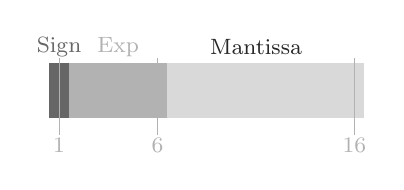
\begin{tikzpicture}[x=0.25cm, y=0.7cm]
        % HALF (16)
        \foreach \i in {0,...,15} {
            \ifnum\i=0
                \fill[gray!80!black] (\i,0) rectangle ++(1,1);
            \else\ifnum\i<6
                \fill[gray!60] (\i,0) rectangle ++(1,1);
            \else
                \fill[gray!30] (\i,0) rectangle ++(1,1);
            \fi\fi
        }
        \node[anchor=center, font=\footnotesize, gray!80!black] at (0.5,1.3) {Sign};
        \node[anchor=center, font=\footnotesize, gray!60] at (3.5,1.3) {Exp};
        \node[anchor=center, font=\footnotesize, gray!30!black] at (10.5,1.3) {Mantissa};
        % Bit position ticks (top)
        \foreach \x/\lbl in {0/1, 5/6, 15/16} {
            \draw[gray!60] (\x+0.5,-0.3) -- (\x+0.5,1.1);
            \node[font=\footnotesize, gray!60] at (\x+0.5,-0.5) {\lbl};
        }
    \end{tikzpicture}
    \caption{Bit layout of IEEE 754 \textbf{HALF (16)}: sign (dark), exponent (medium), mantissa (light).}
    \label{fig:floatformat-half}
\end{figure}

\begin{figure}[h]
    % Requires: \usepackage{tikz}
    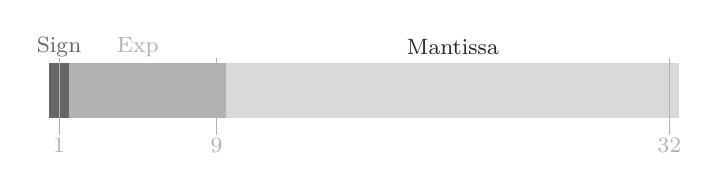
\begin{tikzpicture}[x=0.25cm, y=0.7cm]
        % SINGLE (32)
        \foreach \i in {0,...,31} {
            \ifnum\i=0
                \fill[gray!80!black] (\i,0) rectangle ++(1,1);
            \else\ifnum\i<9
                \fill[gray!60] (\i,0) rectangle ++(1,1);
            \else
                \fill[gray!30] (\i,0) rectangle ++(1,1);
            \fi\fi
        }
        \node[anchor=center, font=\footnotesize, gray!80!black] at (0.5,1.3) {Sign};
        \node[anchor=center, font=\footnotesize, gray!60] at (4.5,1.3) {Exp};
        \node[anchor=center, font=\footnotesize, gray!30!black] at (20.5,1.3) {Mantissa};
        % Bit position ticks (top)
        \foreach \x/\lbl in {0/1, 8/9, 31/32} {
            \draw[gray!60] (\x+0.5,-0.3) -- (\x+0.5,1.1);
            \node[font=\footnotesize, gray!60] at (\x+0.5,-0.5) {\lbl};
        }
    \end{tikzpicture}
    \caption{Bit layout of IEEE 754 \textbf{SINGLE (32)}: sign (dark), exponent (medium), mantissa (light).}
    \label{fig:floatformat-single}
\end{figure}

\begin{figure}[h]
    % Requires: \usepackage{tikz}
    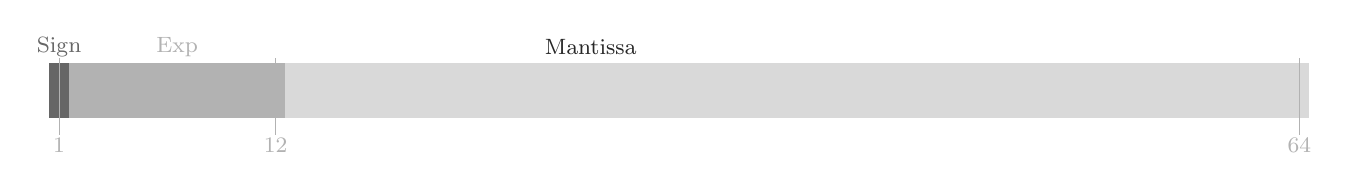
\begin{tikzpicture}[x=0.25cm, y=0.7cm]
        % DOUBLE (64)
        \foreach \i in {0,...,63} {
            \ifnum\i=0
                \fill[gray!80!black] (\i,0) rectangle ++(1,1);
            \else\ifnum\i<12
                \fill[gray!60] (\i,0) rectangle ++(1,1);
            \else
                \fill[gray!30] (\i,0) rectangle ++(1,1);
            \fi\fi
        }
        \node[anchor=center, font=\footnotesize, gray!80!black] at (0.5,1.3) {Sign};
        \node[anchor=center, font=\footnotesize, gray!60] at (6.5,1.3) {Exp};
        \node[anchor=center, font=\footnotesize, gray!30!black] at (27.5,1.3) {Mantissa};
        % Bit position ticks (top)
        \foreach \x/\lbl in {0/1, 11/12, 63/64} {
            \draw[gray!60] (\x+0.5,-0.3) -- (\x+0.5,1.1);
            \node[font=\footnotesize, gray!60] at (\x+0.5,-0.5) {\lbl};
        }
    \end{tikzpicture}
    \caption{Bit layout of IEEE 754 \textbf{DOUBLE (64)}: sign (dark), exponent (medium), mantissa (light).}
    \label{fig:floatformat-double}
\end{figure}
%NTH: Caption should not colide with the plot.


\marginnote{\newthought{A Bit,} short for binary digit, is the most basic unit of information in computing and digital communications. It can have a value of either 0 or 1.}

\newthought{The exponent} is stored with a bias to allow both positive and negative exponents. This allows floating-point numbers to represent both 
very small and very large magnitudes.
For example, in IEEE 754 single precision, the exponent uses 8 bits and a bias of 127. 
The stored exponent $E$ is related to the true exponent $e$ by $e = E - 127_{10}$.
The reason for the bias of 127 is that with 8 bits, the exponent field can store values from 0 ($2^0 - 1$) to 255 ($2^8 - 1$).
By subtracting the bias (127), the actual exponent $e$ can take both positive and negative values, centered around zero. 
This makes encoding and comparison of floating-point numbers easier in hardware.

% NTH: Show how in hardware this means a simple unsigned integer comparison.


\newthought{Constructing scale} in floating-point representation:

\marginnote{
\newthought{The largest number in single precision} is about $10^{38}$, set by the largest exponent $e = +127$. 
The decimal exponent $38$ comes from $\log_{10}(2^{128}) \approx 38.5$.
}

\marginnote{
\newthought{Remember,} mega ($10^6$), giga ($10^9$), tera ($10^{12}$), peta ($10^{15}$), exa ($10^{18}$), zetta ($10^{21}$), yotta ($10^{24}$),
ronna ($10^{27}$), quetta ($10^{30}$), \\
\textbf{no official SI prefix} for ($10^{33}$).}

\begin{align*}
    10^1 &= 10_{10} = 1010_2 = 1.010 \times 2^{3}, \quad \textit{E} = 10000010_2 \\
    10^2 &= 100_{10} = 1100100_2 = 1.100100 \times 2^{6}, \quad \textit{E} = 10000101_2 \\
    10^3 &= 1000_{10} = 1111101000_2 = 1.111101000 \times 2^{9}, \quad \textit{E} = 10001000_2 \\
\end{align*}




\newthought{The mantissa} determines how finely numbers can be represented between powers of two. 

\newthought{2-bit Mantissa Example (unnormalized):}
\begin{align*}
    \text{Mantissa bit combinations:} &\quad 00,\ 01,\ 10,\ 11 \\
    \text{Unnormalized significand:} &\quad 0.xx_2 \\
    \\
    00: \quad 0.00_2 =& 0 + 0 \times 2^{-1} + 0 \times 2^{-2} = 0.0 \\
    01: \quad 0.01_2 =& 0 + 0 \times 2^{-1} + 1 \times 2^{-2} = 0.25 \\
    10: \quad 0.10_2 =& 0 + 1 \times 2^{-1} + 0 \times 2^{-2} = 0.5 \\
    11: \quad 0.11_2 =& 0 + 1 \times 2^{-1} + 1 \times 2^{-2} = 0.75 \\
\end{align*}

\newthought{A two bit mantissa} means we can represent four distinct values between any two powers of two. A three bit mantissa allows eight distinct values, and so on.
In general, with a mantissa of $t$ bits, we can represent $2^t$ distinct values between any two powers of two, scaled up by the exponent.

\newthought{Machine epsilon} ($\varepsilon_{\text{mach}}$) is the smallest positive number such that $1 + \varepsilon_{\text{mach}} \neq 1$ in the computer's arithmetic. It quantifies the upper bound on relative error due to rounding in floating-point arithmetic:

\begin{equation}
    \varepsilon_{\text{mach}} = 2^{-t},
\end{equation}
\index{machine epsilon}

where $t$ is the number of bits in the mantissa. 

\marginnote{For IEEE 754 single precision, $\varepsilon_{\text{mach}} \approx 1.19 \times 10^{-7}$; for double precision, $\varepsilon_{\text{mach}} \approx 2.22 \times 10^{-16}$.
}

In our 2-bit Mantissa example this is: 
\begin{equation*}
    \varepsilon_{\text{mach}} = 2^{-2} = 0.25
\end{equation*}






\marginnote{\newthought{Absolute precision} is just about to become clear, $1:2 = 0.5$ but $10:2 = 5$. 
Same number of steps (relative precision), but gaps of $0.5$ vs $5$.}

\newthought{This means} that the relative precision of floating-point numbers is approximately $2^{-t}$, 
while the absolute precision depends on the magnitude of the number being represented:
\begin{equation}
    \varepsilon_{\text{mach}} \cdot |x|.
\end{equation}

\newthought{In other words} large numbers have larger absolute gaps between representable values than small numbers.

\vspace{3.5em}

\begin{figure}[h]
    \centering
    % Requires: \usepackage{pgfplots}
    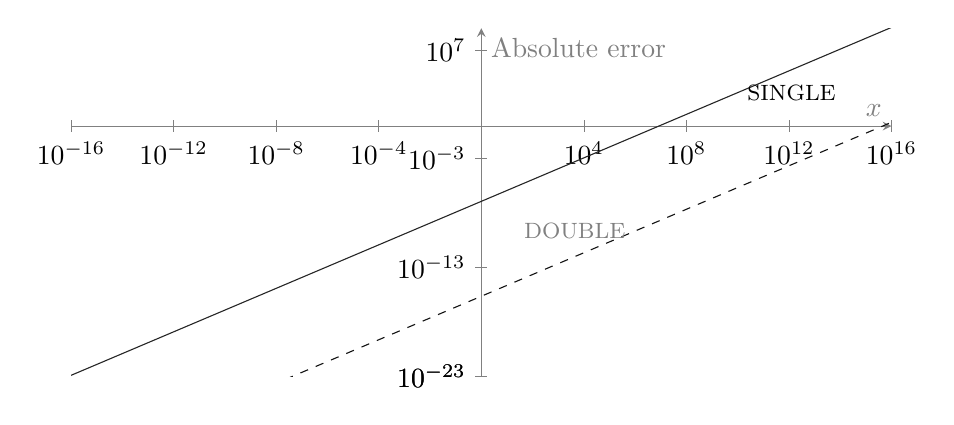
\begin{tikzpicture}
        \begin{axis}[
            width=12cm,
            height=6cm,
            xmode=log,
            ymode=log,
            xlabel={$x$},
            ylabel={Absolute error},
            axis x line=middle,
            axis y line=middle,
            axis line style={gray},
            tick style={gray},
            label style={gray},
            xmin=1e-16, xmax=1e16,
            ymin=1e-23, ymax=1e9, % 
            samples=100,
            domain=1e-16:1e16,
            % No grid, no box, no legend
            extra y ticks={1e-23},
        ]
        % Single precision error envelope (black, solid)
        \addplot[gray!30!black, thin, smooth, domain=1e-16:1e16] {1.19e-7*x};
        % Double precision error envelope (gray, dashed)
        \addplot[gray!15!black, thin, dashed, smooth, domain=1e-16:1e16] {2.22e-16*x};
        % Add labels manually
        \node[anchor=west, font=\footnotesize, black] at (axis cs:1e10,1.19e-7*1e10) {SINGLE};
        \node[anchor=east, font=\footnotesize, gray] at (axis cs:1e6,2.22e-16*1e6) {DOUBLE};
        \end{axis}
    \end{tikzpicture}
    \caption{Absolute error for single (black, labeled SINGLE) and double (gray, dashed, labeled DOUBLE) precision as a function of the represented value $x$. The error grows linearly with $x$ and is proportional to machine epsilon for each format.}\index{absolute error}
    \label{fig:abs_error_float_double}
\end{figure}


% NTH: Also introduce the normalization trick which allows us to win another bit of precision.
%\marginnote{
%\newthought{The normalization trick} introduces an implicitly leading $1$ in the mantissa for non-zero numbers, this number is not stored but assumed.
%}



\index{fixed-point representation}

\newthought{Fixed-point representation}\index{fixed-point representation} is another way to store real numbers in computers, 
especially when you want predictable precision and performance. In fixed-point, you decide in advance how 
many bits are used for the integer part and how many for the fractional part. This means the gap between 
representable numbers (the precision) is always the same, no matter how large or small the value. Which gives more control.

\newthought{Example:} Suppose you want to store numbers between $-1000$ and $1000$ using a 32-bit signed integer. 
Normally, a 32-bit integer can represent values from $-2147483648$ to $2147483647$, which is much more than you need. 
To get more precision, you can use a scaling factor: For example, multiply every real number by $10^6$ and store the 
result as an integer. So, the number $1.234567$ becomes $1234567$ in storage.

\marginnote{\newthought{Precision,} with a scaling factor of $10^{-6}$, is equal to the smallest difference you can represent is $0.000001$. The maximum rounding error is half a step, or $0.5 \times 10^{-6} = 0.0000005$.}







 






% ==============================================================================================
% STUDENT ACTIVATION BLOCK - 15 minutes


\newpage
\section{Examples \& Excercises}




\marginnote{\newthought{Pseudo-Accuracy}\index{pseudo-accuracy} in general is a unjustifiably high level of detail, creating a misleading, and artificial sense of accuracy.}

\newthought{Let's take a closer look} at loss of significance, also called catastrophic cancellation.

This occurs when subtracting two nearly equal numbers, causing leading digits to cancel and leaving only the less significant, rounding-error-prone digits.\index{catastrophic cancellation}\index{loss of significance}
This can greatly amplify rounding errors\index{rounding error}. Let's say we have:
\newthought{Suppose we have two numbers} $a$ and $b$ that are both stored in a computer with limited precision. 
Let’s say each is rounded to 8 significant digits\index{significant digits} as a fixed-point representation\index{fixed-point representation}:

\begin{align*}
    a &= 12345678.5  \\
    b &= 12345678.0 
\end{align*}

But with 8 significant digits, they are stored as:
\begin{align*}
    \tilde{a} &= 12345679 \ \\
    \tilde{b} &= 12345678
\end{align*}

Now, subtract:
\begin{align*}
    \tilde{a} - \tilde{b} &= 12345679 - 12345678 = 1
\end{align*}

Compare to the true difference:
\begin{align*}
    a - b = 12345678.5 - 12345678.0 = 0.5
\end{align*}

\newthought{The error in the result} is $0.5$, which is equal to the rounding error in $\tilde{a}$ or $\tilde{b}$ individually at the machine epsilon level $0.5$.
Let's have a look at what happens with a minimal deviation in the numbers.

\begin{align*}
    a &= 12345678.4  \\
    b &= 12345678.0 
\end{align*}

But with 8 significant digits, they are stored as:
\begin{align*}
    \tilde{a} &= 12345678 \ \\
    \tilde{b} &= 12345678
\end{align*}

Now, subtract:
\begin{align*}
    \tilde{a} - \tilde{b} &= 12345678 - 12345678 = 0
\end{align*}

Compare to the true difference:
\begin{align*}
    a - b = 12345678.4 - 12345678.0 = 0.4
\end{align*}


\marginnote{\newthought{Infinity} in mathematics there is an infinity between 0 and 1. The difference between something and nothing.}
\newthought{The difference in the true results} is $0.1$, but comparing the machine results, we see that the result is $0$ in one case and $1$ in the other,
which is a huge relative error. This shows how loss of significance can lead to large errors in computations, especially when the numbers being subtracted are very close to each other.


\vspace{2em}
\marginnote{\newthought{Code} is again to be found here \url{https://github.com/Quillstacks/lecturecode_numericalmethods.git}.}

\marginnote{\newthought{Overflow,} occurs when numbers with large magnitude are approximated as $+\infty$ or $-\infty$.}
\marginnote{\newthought{Underflow,} occurs when numbers near zero are rounded to zero.}

\newthought{Hands on machine epsilon.} But just before you head over to your machine, think about how you would determine the machine epsilon of any given system, 

for a specific floating-point format, by deploying a program. Revisit how machine epsilon\index{machine epsilon} is defined. Write down your thoughts in pseudo-code. 
What would such a program show when run on a fixed-point system\index{fixed-point representation} vs a floating-point system\index{floating-point representation}? Write down your thoughts. Then try different types on your machine in code.
Write down things that you observe and reflect on them. 

\marginnote{\newthought{Is double enough?}}
When you would build a calculator, which type would you choose and why \cite{blochingerfoliensatz}?\index{numerical stability}




\newthought{Loss of significance example.} Now, think about how you would demonstrate loss of significance on your machine. 
Write down your thoughts in pseudo-code, before you read beyond this point.
\vspace{2em}


\begin{figure}[h]

    \centering
    % Requires: \usepackage{pgfplots}
    \begin{tikzpicture}
        \begin{axis}[
            width=13cm,
            height=6cm,
            xmode=log,
            xlabel={$\epsilon$},
            ylabel={$1/(1+\epsilon-1)$},
            axis x line=bottom,
            axis y line=left,
            tick style={gray},
            label style={gray},
            axis line style={gray},
            xmin=1e-17, xmax=1e-14,
            ymin=0, ymax=2e16,
            extra x ticks={1e-16,1e-15,1e-14},
            extra x tick style={
                grid=major,
                major grid style={draw=gray!10, very thin},
                tick label style={gray}
            },
            grid=none,
        ]
        % Reference line: y = 1/epsilon
        \addplot[gray!30!black, solid, domain=1e-17:1e-14, samples=100] {1/x};
        % Add label showing curve goes to infinity
        \node[font=\footnotesize, anchor=center, fill=white, text=black] at (axis cs:4e-17,1.9e16) {$\uparrow$ $\infty$};
        \end{axis}
    \end{tikzpicture}
    \caption{Demonstration of catastrophic loss of significance: $1/(1+\epsilon-1)$ vs $\epsilon$ (log-x, linear-y scale).
    For large $\epsilon$, the result follows $1/\epsilon$. For very small $\epsilon$, rounding error dominates and the result
    becomes infinite.}\index{catastrophic cancellation}\index{loss of significance}\index{rounding error}
    \label{fig:catastrophic_loss_significance}
\end{figure}

\marginnote{
\newthought{What happens} for $a > b$? \\
Think along the lines of significant digits.}

\newthought{Reason about} how computing $f(\epsilon) = 1 / (a + \epsilon - b)$ for small $\epsilon$ and $a = b$ would do the job.
What do you expect to see when $\epsilon$ is very small?



\section{Self-Reflection and Recap}

%<Discussion about the findings and the learned concepts>
\newthought{Self-Reflection} Questions which can guide your thoughts during the excercises and afterwards:\index{floating-point representation}\index{machine epsilon}\index{numerical stability}
\begin{itemize}
    \item How is floating-point representation\index{floating-point representation} structured, and what are its components?
    \item What is machine epsilon\index{machine epsilon}, and how does it relate to numerical precision?\index{significant digits}
    \item How do these concepts impact numerical computations in practice?\index{numerical stability}
\end{itemize}

%<Recap of Key Concepts>
\newthought{Recap} of Key Concepts:\index{floating-point arithmetic}\index{machine epsilon}\index{loss of significance}
\begin{itemize}
    \item Floating-point representation\index{floating-point representation} allows computers to store a wide range of real numbers using a finite number of bits, but introduces rounding errors\index{rounding error}.
    \item Machine epsilon\index{machine epsilon} quantifies the smallest difference that can be represented in floating-point arithmetic, affecting the precision of numerical computations.\index{significant digits}
    \item Loss of significance\index{loss of significance} occurs when subtracting nearly equal numbers, amplifying rounding errors\index{rounding error} and leading to inaccurate results.\index{catastrophic cancellation}
\end{itemize}


\marginnote{\newthought{Teaser.} Can you think of metrics for numerical methods, based on the approximations and errors we discussed?\index{grid search}}

\newthought{Knowing what can go wrong.} We are now close to understanding how we can define what is good and the quality of our methods. 
We now know that there is a true function $f$ and an approximated function $\tilde{f}$, 
further we have a true input $x$ and a rounded input $\tilde{x}$. These effect and characterize our numerical methods.\index{modeling error}\index{pseudo-accuracy}






%%%%%%%%%%%%%%%%%%%%%%%%%%%%%%%%%%%%%%%%%%%%%%%%%%%%%%%%%%%%%%%%%%%%%%%%%%%%%%







































